%----------------------------------------------------------------------------------------
%	PACKAGES AND DOCUMENT CONFIGURATIONS
%----------------------------------------------------------------------------------------

\documentclass[9pt,twocolumn]{article}

\usepackage{hyperref}
\usepackage{caption}
\usepackage{graphicx} % Required for the inclusion of images
\usepackage{amsmath} % Required for some math elements 
\usepackage[margin=30mm]{geometry}

\usepackage{color} %red, green, blue, yellow, cyan, magenta, black, white
\definecolor{mygreen}{RGB}{28,172,0} % color values Red, Green, Blue
\definecolor{mylilas}{RGB}{170,55,241}

\usepackage{listings}
\lstset{language=Matlab,
    basicstyle=\ttfamily,
    breaklines=true       
}

\captionsetup[figure]{font=small}
\addtolength{\topmargin}{-16mm}
\addtolength{\textheight}{32mm}


\setlength\parindent{0pt} % Removes all indentation from paragraphs
\renewcommand{\labelenumi}{\alph{enumi}.} % Make numbering in the enumerate environment by letter rather than number (e.g. section 6)

%----------------------------------------------------------------------------------------
%	DOCUMENT INFORMATION
%----------------------------------------------------------------------------------------

\title{ECEN 220 \\ Lab Report 2 - Fourier Series}
\author{Daniel Eisen : 300447549}
\date{\today}

\begin{document}
\maketitle

\section{Harmonic Convergence}
\lstinputlisting{q1.m}
\begin{figure}[h]
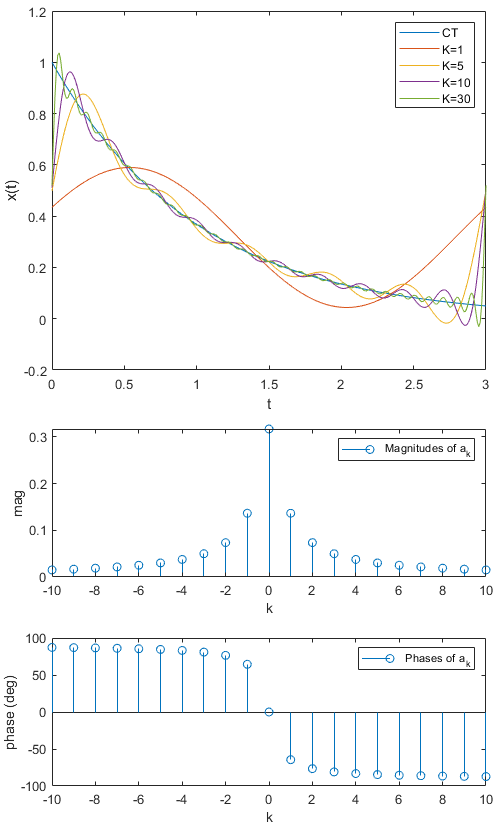
\includegraphics[width=0.5\textwidth]{1}
\caption{FS}
\end{figure}

\clearpage
\section{Average Signal Power}
\lstinputlisting{q2.m}
\newpage
\begin{figure}[h]
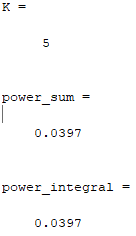
\includegraphics[width=0.3\textwidth]{2}
\caption{SP}
\end{figure}
\end{document}